
Nous rappelons que la fonction de co\^ut est d\'efinie par la somme des co\^uts des cases \`a modifier pour corriger chaque sommet de $\cal C$ pendant l'algorithme de correction. 
Le co\^ut de correction d'un sommet est le co\^ut minimal de toutes les cases modifi\'ees. 
Nous recherchons alors la fonction de co\^ut qui minimise globalement le co\^ut de correction des sommets de $\cal C$.
Pour ce faire, nous comparons d'abord les fonctions de co\^ut {\em unitaire} et {\em normale} parce que nous souhaitons savoir s'il est pr\'ef\'erable d'utiliser les valeurs de corr\'elations dans les co\^uts des op\'erations. Puis nous comparons la meilleure des deux fonctions avec celles {\em ajout} et {\em suppression}.
La figure \ref{comparaisonFctCoutUnitaireNormale} contient 
\begin{itemize}
	\item La comparaison des distances de Hamming entre les  fonctions de co\^ut {\em unitaire} et {\em normale} (graphique $(e)$).
	\item La comparaison du nombre de cases {\em fausses n\'egatives} entre les deux fonctions de co\^ut avant l'algorithme de correction (graphique $(b)$).
	\item  La comparaison du nombre de cases {\em fausses n\'egatives} entre les deux fonctions de co\^ut apr\`es l'algorithme de correction (graphique $(d)$).
	\item La comparaison du nombre de cases {\em fausses positives} entre les deux fonctions de co\^ut avant l'algorithme de correction (graphique $(a)$).
	\item  La comparaison du nombre de cases {\em fausses positives} entre les deux fonctions de co\^ut apr\`es l'algorithme de correction (graphique $(a)$).
\end{itemize}
Les distances de Hamming et les nombres de cases sont ordonn\'ees par ordre croissant.

% ----------- comparaisonFctCoutNormaleAjoutSuppression -----------------
\vspace{-0.5cm}
\begin{figure}[htb!] 
\centering
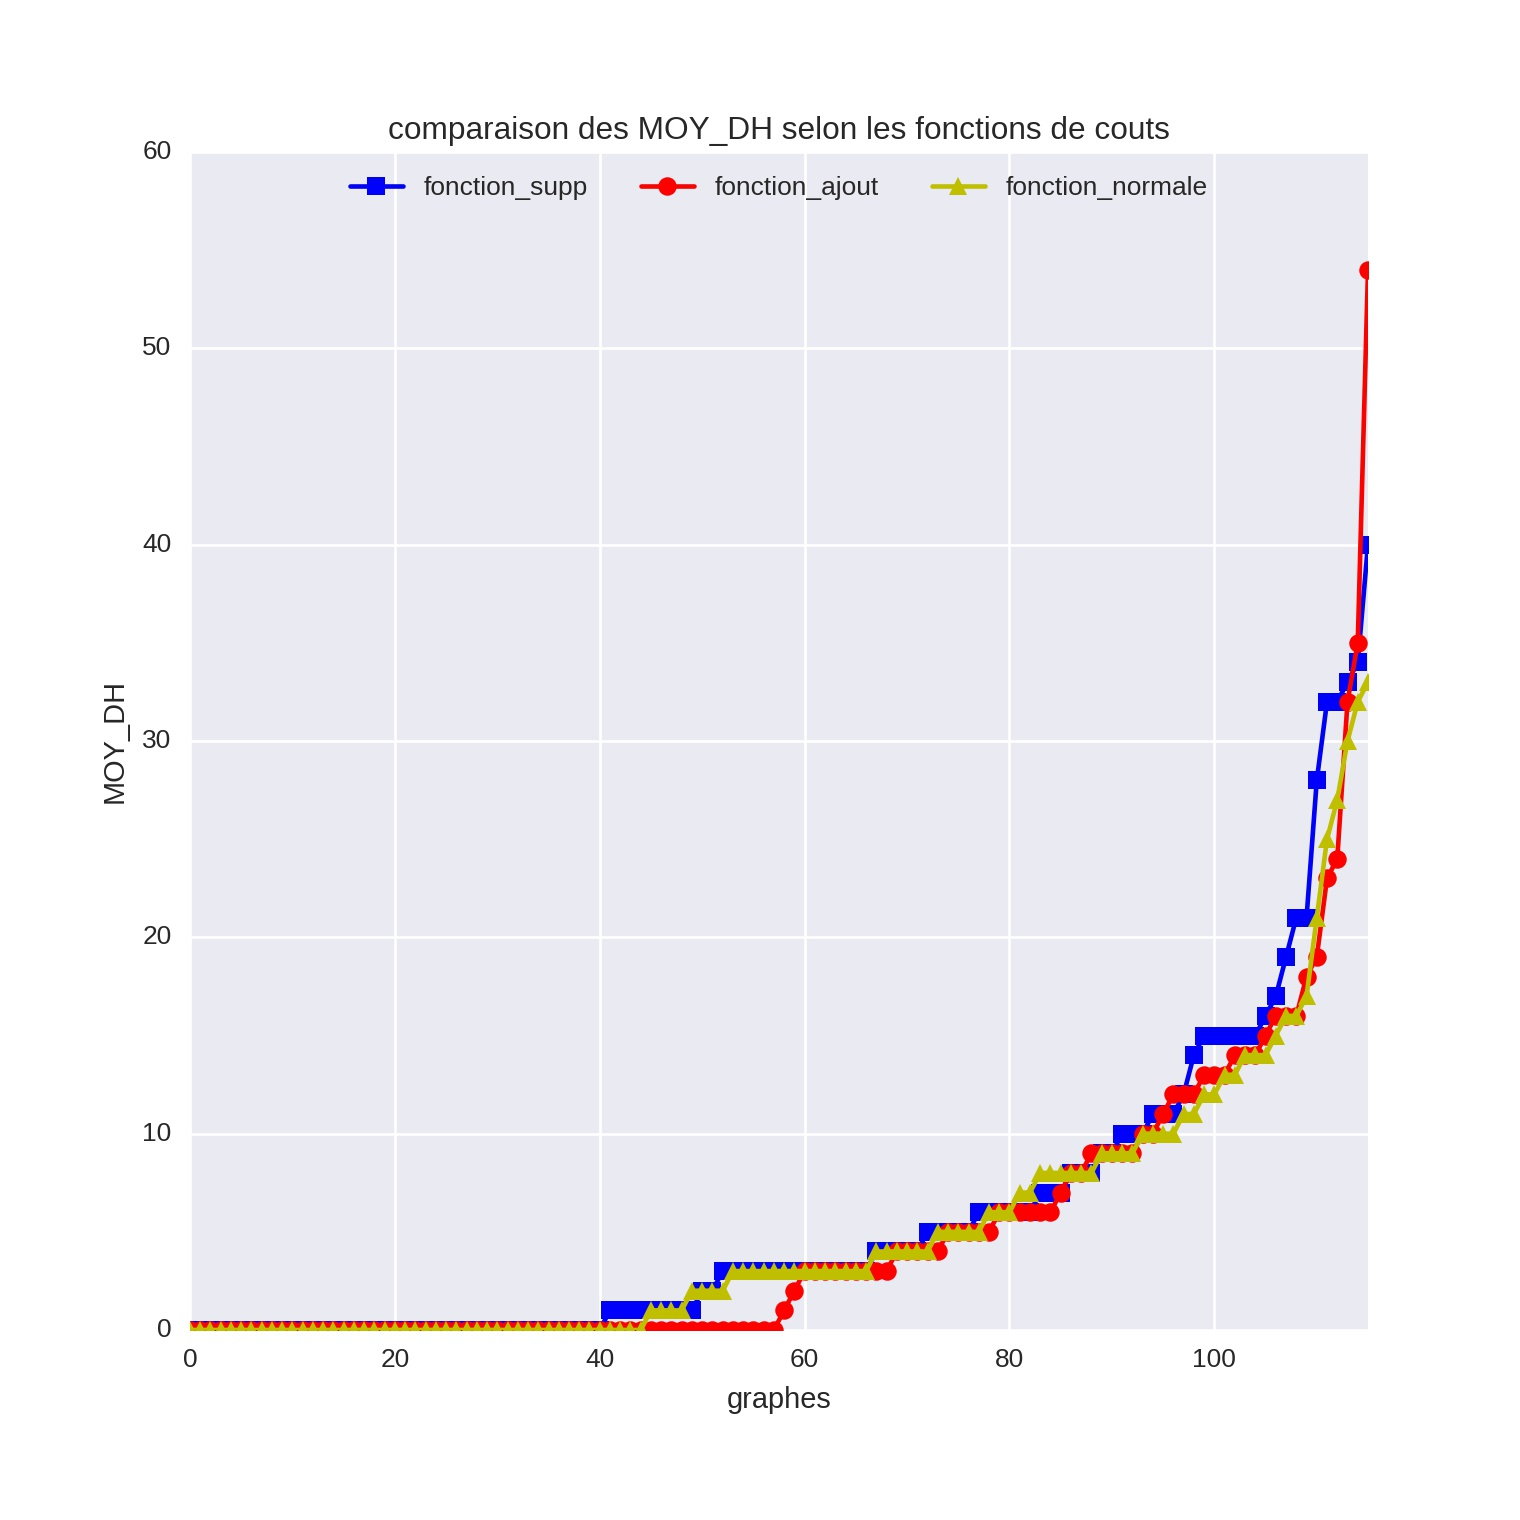
\includegraphics[scale=0.25]{comparaison_fct_couts_moy_dh_s_07_aleatoire_supp_ajout_normale.jpeg}
\caption{ Comparaison entre les fonctions de co\^ut {\em normale},  {\em ajout} et  {\em suppression} : la fonction {\em ajout} est la courbe en rouge, la fonction {\em normale} est en jaune et la fonction {\em suppression est en bleu}}
\label{comparaisonFctCoutNormaleAjoutSuppression} 
\end{figure}
 \FloatBarrier
% ----------- comparaisonFctCoutNormaleAjoutSuppression -----------------
Nous constatons que la courbe de la fonction {\em unitaire} est au dessus de celle de la fonction {\em normale} dans le graphique $(e)$ de la figure \ref{comparaisonFctCoutUnitaireNormale}.
Avec $s=0.7$, l'ensemble de cases erron\'ees sont des cases {\em fausses positives} (graphique $(c)$ de la figure \ref{comparaisonFctCoutUnitaireNormale}).
En appliquant les fonctions {\em unitaire} et {\em normale}, nous avons l'introduction de cases {\em fausses n\'egatives} et le nombre de ces cases est plus important dans la fonction {\em unitaire}. Ce nombre fait cro\^itre la distance de Hamming $moy\_DH$ parce que la correction a r\'eduit le nombre de cases {\em fausses positives} dans la fonction {\em normale} (voir les graphiques $(a)$ et $(c)$ de la figure  \ref{comparaisonFctCoutUnitaireNormale}).
Ce qui explique les faibles distances $moy\_DH$ de la fonction {\em normale}. La fonction {\em normale} donne de meilleurs r\'esultats et nous la choisissons dans le calcul des co\^uts de correction.
\newline

Par ailleurs, dans la figure \ref{comparaisonFctCoutNormaleAjoutSuppression}, les courbes des  fonctions  {\em normale}, {\em ajout} et {\em suppression} sont entremel\'ees et il ne se d\'egage aucun \'ecart significatif entre elles. Il est donc difficile de juger l'influence d'une des fonctions sur la correction des sommets de $\cal C$.  
\newline 

{\bf Conclusion} :
 prioriser l'ajout \`a la suppression et vice versa n'a aucune influence sur les distances de Hamming quand nous utilisons les valeurs de corr\'elations. Toutefois,  il est pr\'ef\'erable de consid\'erer les corr\'elations dans le calcul du co\^ut de la modification d'une case parce que cela am\'eliore les distances $moy\_DH$ comme il est indiqu\'e dans le graphique $(e)$  de la figure \ref{comparaisonFctCoutUnitaireNormale}.